\documentclass[11pt]{amsart}
%\pagestyle{empty} 
\setlength{\topmargin}{-0.5in} % usually -0.25in
\addtolength{\textheight}{1.7in} % usually 1.25in
\addtolength{\oddsidemargin}{-0.95in}
\addtolength{\evensidemargin}{-0.95in}
\addtolength{\textwidth}{1.9in} %\setlength{\parindent}{0pt}

\newcommand{\normalspacing}{\renewcommand{\baselinestretch}{1.1}\tiny\normalsize}
\normalspacing

% macros
\usepackage{amssymb,xspace,alltt,verbatim}
\usepackage[final]{graphicx}
\usepackage[pdftex,colorlinks=true]{hyperref}
\usepackage{fancyvrb}
\usepackage{tikz}

\newtheorem*{lem*}{Lemma}

\newcommand{\ba}{\mathbf{a}}
\newcommand{\bb}{\mathbf{b}}
\newcommand{\bc}{\mathbf{c}}
\newcommand{\bd}{\mathbf{d}}
\newcommand{\bs}{\mathbf{s}}
\newcommand{\bu}{\mathbf{u}}
\newcommand{\bv}{\mathbf{v}}
\newcommand{\bw}{\mathbf{w}}
\newcommand{\bx}{\mathbf{x}}
\newcommand{\by}{\mathbf{y}}

\newcommand{\bbf}{\mathbf{f}}

\newcommand{\bV}{\mathbf{V}}
\newcommand{\bW}{\mathbf{W}}

\newcommand{\CC}{{\mathbb{C}}}
\newcommand{\RR}{{\mathbb{R}}}
\newcommand{\eps}{\epsilon}
\newcommand{\ZZ}{{\mathbb{Z}}}
\newcommand{\ZZn}{{\mathbb{Z}}_n}
\newcommand{\NN}{{\mathbb{N}}}
\newcommand{\ip}[2]{\mathrm{\left<#1,#2\right>}}

\renewcommand{\Re}{\operatorname{Re}}
\renewcommand{\Im}{\operatorname{Im}}

\newcommand{\Log}{\operatorname{Log}}

\newcommand{\Span}{\operatorname{span}}

\newcommand{\grad}{\nabla}

\newcommand{\ds}{\displaystyle}

\newcommand{\Matlab}{\textsc{Matlab}\xspace}
\newcommand{\Octave}{\textsc{Octave}\xspace}
\newcommand{\pylab}{\textsc{pylab}\xspace}

\newcommand{\prob}[1]{\bigskip\noindent\textbf{#1.} }
\newcommand{\pts}[1]{(\emph{#1 pts})}

\newcommand{\probpts}[2]{\prob{#1} \pts{#2} \quad}
\newcommand{\ppartpts}[2]{\textbf{(#1)} \pts{#2} \quad}
\newcommand{\epartpts}[2]{\medskip\noindent \textbf{(#1)} \pts{#2} \quad}

\newcommand{\mybox}{\boxed{\phantom{\begin{bmatrix} I & I \\ O & O \end{bmatrix} fj ladsfj}}}
\newcommand{\dbox}{\boxed{\phantom{\begin{bmatrix} I & I \\ O & O \end{bmatrix}}}}


\begin{document}
\hfill \Large Name:\underline{\phantom{Ed Bueler really really long long long name}}
\medskip

\scriptsize \noindent Math 314 Linear Algebra (Bueler) \hfill Friday, 29 April 2022
\medskip

\LARGE\centerline{\textbf{Final Exam}}

\smallskip
\begin{quote}
\large
\textbf{No book, electronics, calculator, or internet access.  Allowed notes: one sheet of letter paper ($=8.5''\times 11''$ paper), with anything written on both sides.  150 points possible.  125 minutes maximum.}
\end{quote}

\normalsize
\medskip

\thispagestyle{empty}

\prob{1}  Consider this $3\times 5$ matrix and its row-reduced echelon form ($R=$\,\texttt{rref(A)}):
    $$A = \begin{bmatrix} 0 & 1 & 2 & 0 & -1 \\
                          0 & 2 & 4 & 0 & -2 \\
                          0 & 0 & 1 & 1 & 2 \end{bmatrix}
      \qquad \to \qquad
      R = \begin{bmatrix} 0 & 1 & 0 & -2 & -5 \\
                          0 & 0 & 1 & 1 & 2 \\
                          0 & 0 & 0 & 0 & 0 \end{bmatrix}$$

\medskip
\epartpts{a}{3}  What is the rank of $A$?
\bigskip\medskip

\epartpts{b}{3}  What is the dimension of the null space of $A$?
\bigskip\medskip

\epartpts{c}{7}  Find a basis for each of these 3 subspaces associated to $A$:
    $$\text{row space } C(A^\top), \quad \text{column space } C(A), \quad \text{null space } N(A)$$
\vfill

\epartpts{d}{5}  

\noindent Fill-in the \textbf{6 bold boxes}

\noindent in the ``big picture'' at right.

\noindent Give either the name of the

\noindent subspace or the dimension

\noindent which applies to the specific

\noindent matrix $A$:

\vspace{-35mm}
\hfill
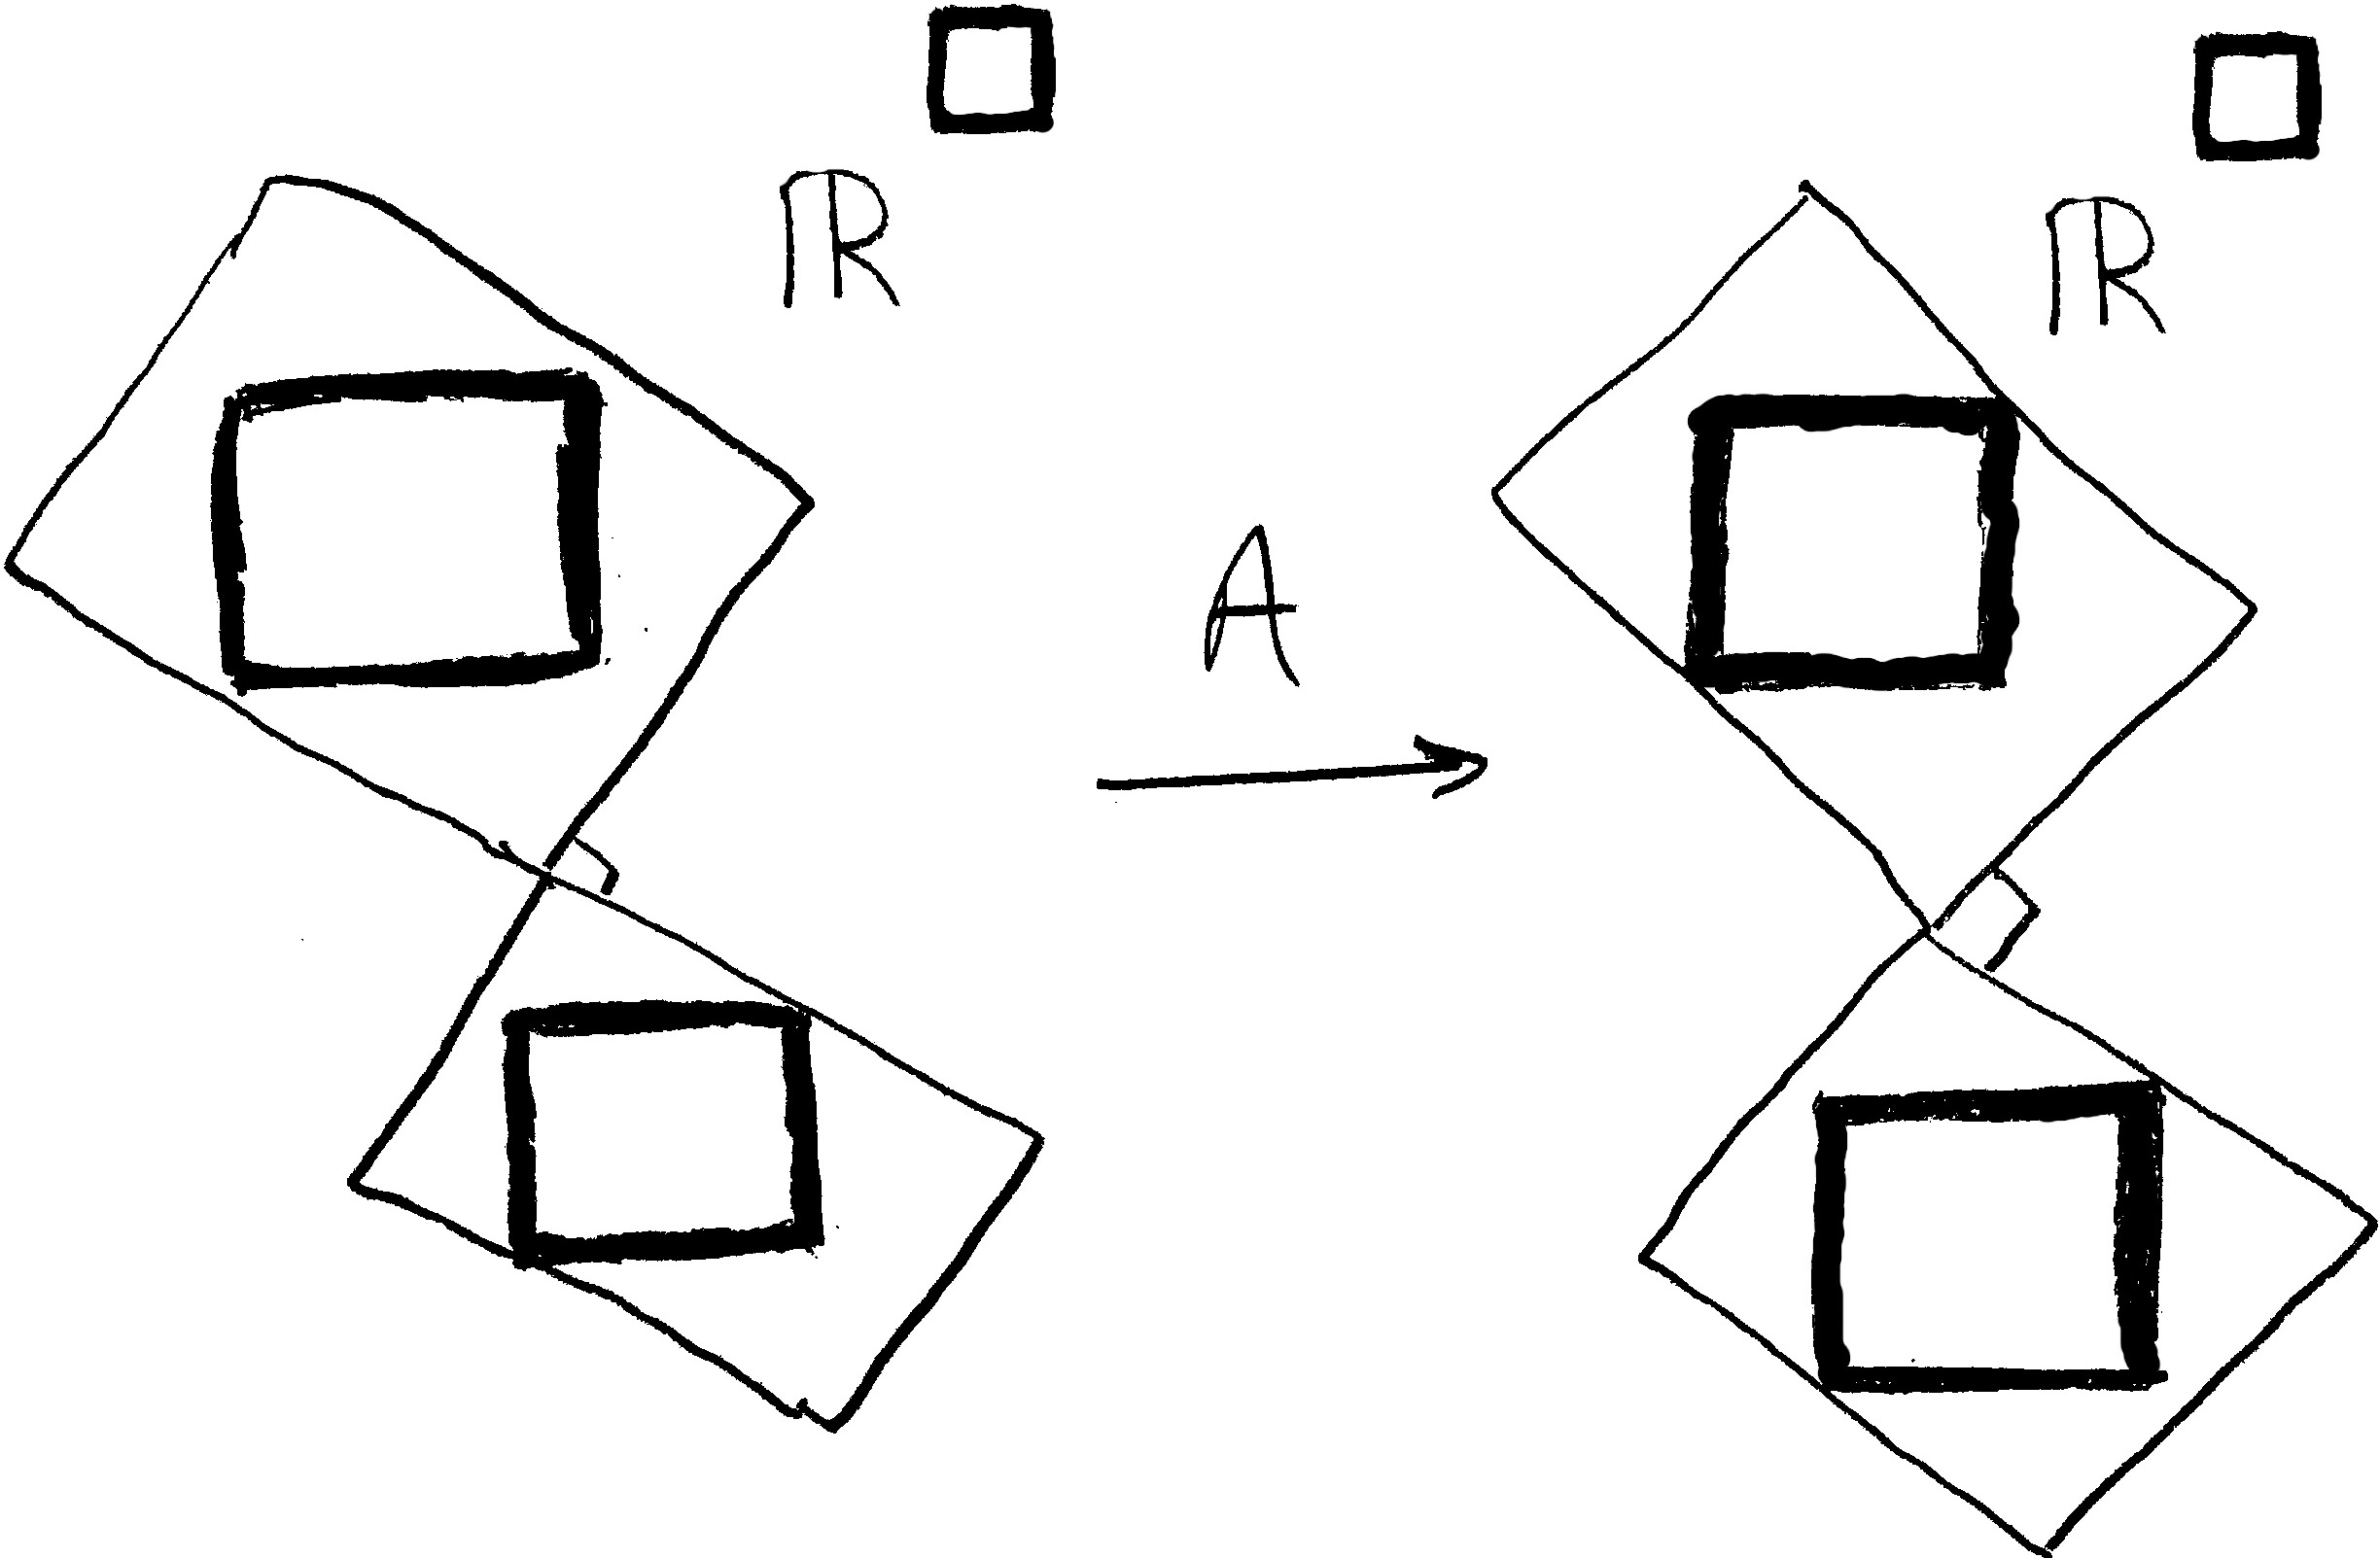
\includegraphics[height=2.7in]{figs/big-pic-by-hand.jpg}


\clearpage \newpage
\prob{2}  Suppose $A$ is any $m$ by $n$ matrix.

\epartpts{a}{7}  Show that the null space $N(A)$ is a subspace.
\vfill

\epartpts{b}{7}  Show that the null space $N(A)$ and the row space $C(A^\top)$ are orthogonal.
\vfill

%older: system of 2 equations not invertible; write general solution
\probpts{3}{7}  Find the general solution of this linear system of two equations, and show your work:
\begin{align*}
3 x_1 - x_2 &= 4 && \hspace{4.0in} \\
-6 x_1 + 2 x_2 &= -8
\end{align*}
\vfill


\clearpage \newpage
\prob{4} \ppartpts{a}{10}  Use the Gauss-Jordan elimination to compute the inverse of

\medskip
\noindent $\ds A = \begin{bmatrix} 1 & 2 & 3 \\ -2 & -2 & -6 \\ 1 & 4 & 4 \end{bmatrix}$.  \,Show your work.
\vfill

\epartpts{b}{5}  At the first stages of elimination in part \textbf{(a)} you applied row operations which can be written as elimination matrices.  Specifically, give the matrices $E_{21}$ and $E_{31}$ which you used.
\vspace{2.0in}


\clearpage \newpage
\prob{5}  Is each statement about square matrices \textbf{True} or \textbf{False}?  \underline{\textbf{If False, provide a counterexample.}}

\epartpts{a}{3}  If $Q$ is an orthogonal matrix then $Q$ is invertible.
\vfill

\epartpts{b}{3}  If $P$ is a projection matrix then $P$ is invertible.
\vfill

\epartpts{c}{3}  If $P$ is a permutation matrix then $P$ is invertible.
\vfill

\epartpts{d}{3}  If $A$ is a diagonalizable matrix then $A$ is invertible.
\vfill

\epartpts{e}{3}  If all eigenvalues of a matrix $A$ are zero then $A=0$.
\vfill

\epartpts{f}{3}  If any eigenvalue of $A$ is zero then $A$ is not invertible.
\vfill

\epartpts{g}{3}  If $A^2=0$ then $A=0$.
\vfill


\clearpage \newpage
\prob{6} \ppartpts{a}{10}  Form and solve the normal equations:.  Show your work.
    $$A = \begin{bmatrix} 1 & -1 \\ 1 & 0 \\ 2 & 0 \\ 2 & -1 \end{bmatrix}, \qquad \bb = \begin{bmatrix} 0 \\ 1 \\ 0 \\ 1 \end{bmatrix} \hspace{4.0in}$$
\vfill

\epartpts{b}{4}  In part \textbf{(a)}, is the vector $\bb$ in the subspace $C(A)$?  Explain your reasoning.
\vspace{2.0in}


\clearpage \newpage
\probpts{7}{7}  Recall that the projection matrix $P$ which projects onto the column space $C(A)$ of a matrix $A$ with linearly-independent columns (full column rank) is $P=A (A^\top A)^{-1} A^\top$.  Show that $P$ is a projection matrix.
\vfill

\prob{8} \ppartpts{a}{7}  Suppose that a square matrix $B$ is diagonalizable, that is, suppose $B = X \Lambda X^{-1}$ where $X$ is invertible and $\Lambda$ is diagonal.   Give a formula which shows why it is easy to compute $B^{100}$.
\vfill

\epartpts{b}{7}  Describe how to compute $\det(B)$ if $B = X \Lambda X^{-1}$ is diagonalized.
\vfill


\clearpage \newpage
\probpts{9}{7}  Let $\ds Q = \begin{bmatrix} 1/2 & -\sqrt{3}/2 \\ -\sqrt{3}/2 & -1/2 \end{bmatrix}$.  Show that $Q$ is an orthogonal matrix.
\vfill

\prob{10} \ppartpts{a}{5}  Recall that $2$ by $2$ rotation matrices have the form
    $$A = \begin{bmatrix} \cos \theta & - \sin \theta \\ \sin \theta & \cos \theta \end{bmatrix}$$
Using this form, find a non-identity matrix $A$ with the property that {\large $A^4=I$}, and verify this property for your matrix.
\vfill

\epartpts{b}{5}  Compute the eigenvalues of the matrix $A$ which you found in part \textbf{(a)}.
\vfill


\clearpage\newpage
\prob{11} \ppartpts{a}{10}  Find the eigenvalues and eigenvectors of the matrix
    $$A = \begin{bmatrix} 2 & 2 & 2 \\ 2 & 0 & 0 \\ 2 & 0 & 0 \end{bmatrix}. \hspace{5.0in}$$
\vfill

\epartpts{b}{3}  Is the matrix in part \textbf{(a)} diagonalizable?  Give a brief justification.  (\emph{Hint.} No further calculations are necessary.)
\vspace{1.5in}


\clearpage\newpage
\prob{12}  Consider the transformations from $\bV=\RR^2$ to $\bW=\RR^2$.  For each one, is it linear?  (\emph{Show it is, or give a counterexample.})  Then give a simplified formula for $T(T(\bv))$.

\epartpts{a}{5}   $T(\bv) = -\bv + (1,1)$
\vfill

\epartpts{b}{5}   $T(\bv) = \frac{1}{2} (v_1+v_2,v_1+v_2)$
\vfill

\noindent \hrulefill
\begin{center}
\small
\textsc{blank space}
\end{center}
\vspace{2.0in}


\clearpage\newpage
\probpts{Extra Credit}{3}  The matrix $\ds Q = \begin{bmatrix} 1/2 & -\sqrt{3}/2 \\ -\sqrt{3}/2 & -1/2 \end{bmatrix}$ in problem \textbf{8} is neither a rotation matrix nor a reflection matrix.  But it can be factored into the product of a rotation matrix and a reflection matrix.  Do so.
\vfill

\noindent \hrulefill
\begin{center}
\small
\textsc{blank space}
\end{center}
\vspace{3.0in}

\end{document}
